\subsection{Abstract Factory Method}
\subsubsection{Định nghĩa}
Abstract Factory Method là một Pattern dùng để tạo ra tập hợp các objects liên quan với nhau mà không cần phải làm rõ các class thành phần.
\subsubsection{Cách sử dụng}
Ta thông thường sử dụng Abtract Factory Method trong các trườn g hợp sau:
\begin{itemize}
    \item 1. Bạn muốn tạo ra một nhóm các Object có liên quan với nhau, hỗ trợ một loạt chức năng liên quan.
    2. Bạn muốn đảm bảo rằng các Objet được tạo ra phù hợp với nhau và tuân thủ các quy tắc nhất định.
    \item 3. Bạn muốn ẩn thông tin về cách tạo ra các Object cụ thể và chỉ tương tác thông qua giao diện chung.
\end{itemize}
\subsubsection{Cấu trúc}
Đầu tiên, ta cần gom tất cả các sản phẩm chung loại vào một lớp interface. Sau đó, ta cần tạo ra một Abstract Factory có chứa toàn bộ các phương thức để tạo ra các loại sản phẩm khác nhau.\\
Với mỗi sản phẩm trong cùng 1 loại, ta tạo ra các Factory cho riêng nó chứa các phương thức để tạo ra các kiểu sản phẩm của loại sản phẩm đó.\\
\newline
\begin{center}
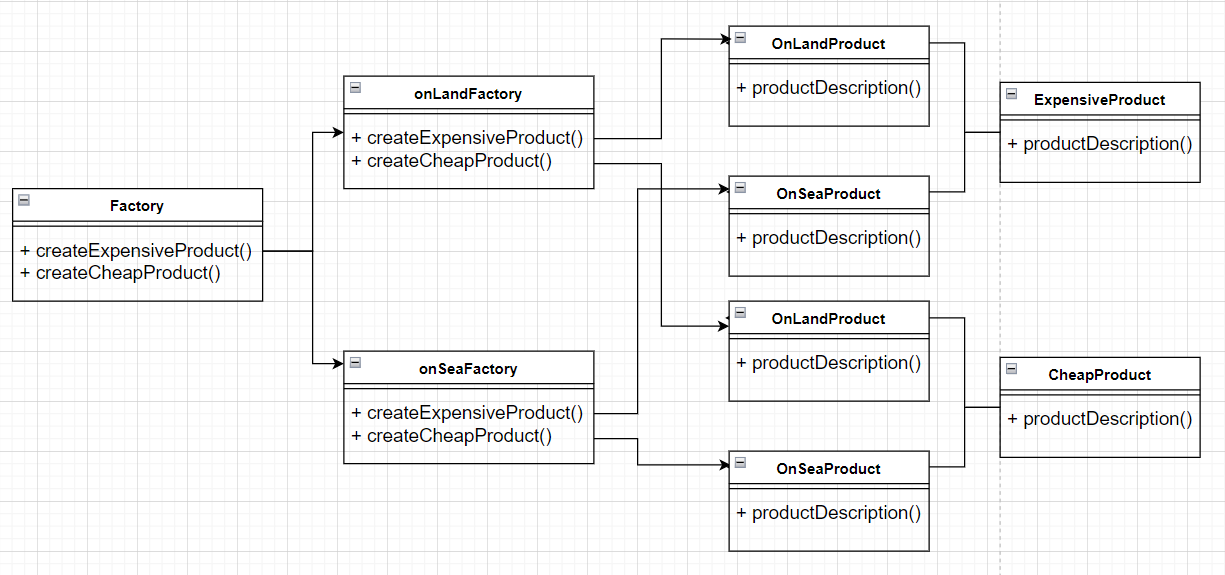
\includegraphics[scale=0.60]{image/creational/afso.png}
\end{center}
Các thành phần chính trong mô hình:
\begin{itemize}
    \item Một interface hoặc abstract class chứa các phương thức để tạo ra các đối tượng sản phẩm.
    \item Các class kế thừa từ interface có nhiệm vụ cài đặt, thực hiện các phương thức tạo nên sản phẩm. Mỗi một class tương ứng chỉ tạo ra duy nhất một loại sản phẩm.
    \item Một interface hoặc abstract class cho một tập hợp các loại sản phẩm liên quan với nhau.
    \item Một loạt các loại sản phẩm liên quan đến nhau kế thừa từ class interface trên.
\end{itemize}
\subsubsection{Ưu điểm và Nhược điểm}
Ta thường thấy một số ưu nhược điểm như sau:\\\\
Ưu điểm:
\begin{itemize}
    \item Nhìn chung Abtract Factory Method hoàn toàn giống với Factory Method ngoài độ ứng dụng với các chương trình lớn ra.
\end{itemize}
Nhược điểm:
\begin{itemize}
    \item Sử dụng Abstract Factory method yêu cầu bạn xây dựng các lớp Factory và Concrete Factory cụ thể. Điều này có thể tạo ra sự phụ thuộc cao giữa các lớp và làm cho mã khó hiểu hơn nếu không được sử dụng một cách hợp lý.
    \item Việc tạo ra các đối tượng thông qua Abstract Factory có thể tạo ra tiềm ẩn lỗi nếu không xử lý tốt việc tạo đối tượng.
\end{itemize}
\subsubsection{Code}
\begin{itemize}
    \item Chúng ta có 2 loại sản phẩm là sản phẩm đắt tiền và sản phẩm rẻ hơn.
    \item Ở sản phẩm đắt, ta có 2 loại là Xe hơi và Du thuyền. Còn đối với loại sản phẩm rẻ tiền hơn, ta có Xe đạp và Thuyền.
    \item Ta có 2 loại nhà máy là nhà máy sản xuất các phương tiện trên bờ và nhà máy sản xuất các phương tiện trên mặt nước.
\end{itemize}

\begin{lstlisting}
#include <iostream>
using namespace std;

//--------------------------------------
class ExpensiveProduct
{
public:
    virtual void productDescription() = 0;
};

class CheapProduct
{
public:
    virtual void productDescription() = 0;
};
//--------------------------------------
class Bike : public CheapProduct
{
public:
    void productDescription() override { cout << "Bike" << endl; }
};

class Boat : public CheapProduct
{
public:
    void productDescription() override { cout << "Boat" << endl; }
};

class Car : public ExpensiveProduct
{
public:
    void productDescription() override { cout << "Car" << endl; }
};

class Yatch : public ExpensiveProduct
{
public:
    void productDescription() override { cout << "Yatch" << endl; }
};
//--------------------Factory---------------------
class Factory
{
public:
    virtual CheapProduct *createCheapProduct() = 0;
    virtual ExpensiveProduct *createExpensiveProduct() = 0;
};
//------------------------------------------------
class onLandFactory : public Factory
{
public:
    ExpensiveProduct *createExpensiveProduct() override { return new Car; };
    CheapProduct *createCheapProduct() override { return new Bike; };
};

class onSeaFactory : public Factory
{
public:
    ExpensiveProduct *createExpensiveProduct() override { return new Yatch; };
    CheapProduct *createCheapProduct() override { return new Boat; };
};
//-----------------------------------------------

int main()
{
    Factory *f1 = new onLandFactory();
    f1->createCheapProduct()->productDescription();
    f1->createExpensiveProduct()->productDescription();
    Factory *f2 = new onSeaFactory();
    f2->createCheapProduct()->productDescription();
    f2->createExpensiveProduct()->productDescription();
}
\end{lstlisting}
Ở hàm main, ta tạo ra nhà máy sản xuất phương tiện di chuyển trên mặt đất rồi sản xuất lần lượt các sản phẩm đắt tiền và rẻ tiền, tương tự với nhà máy sản xuất phương tiện di chuyển trên mặt nước.\\
\newline
\textbf{Kết quả:}
\begin{lstlisting}
Bike
Car
Boat
Yatch
\end{lstlisting}
\subsubsection{Các Pattern liên quan}
\begin{itemize}
    \item Factory Method: đây là nguồn gốc để phát triển lên được Abstract Factory.
    \item Builder: có thể kết hợp với Builder để chạy một vài bước tạo sản phẩm trước khi Abstract Factory trả về sản phẩm.
    \item Prototype: đương nhiên việc mỗi class khởi tạo của Abstract Factory có thêm một hàm clone() cũng không phải việc gì quá khó khăn.
    \item Singleton: hoặc là ta có thể làm cho các đối tượng mà Abstract Factory tạo là là duy nhất và được truy cập từ khắp nơi trên mã nguồn.
\end{itemize}
